\setcounter{chapter}{12-1} %Makes the prereq chapter chapter 0

\chapter{Markov Decision Processes 0 - State Machines}

\setcounter{section}{0}

\section{State Machines}

    \subsection{How to Model Time}

        How do we want to model time?

        The simplest way is one we've used before: keeping track of the current \gren{timestep} $t$.

        \begin{itemize}
            \item But this is too little information to be useful: it doesn't tell us much.
            \item \miniex If I told you "the current time is $t=1563$", that doesn't help you much with decision-making.
        \end{itemize}

        So, what would be a \textbf{useful} representation of time? We've already shown that we don't really care much about the exact \textbf{index} of time $t$.

        Instead, we care about \gren{what happened} in the past.\\

        \begin{concept}
            One simple way to record the past is to ask about \gren{events}, and \purp{when} they happened.
        \end{concept}

        \miniex You might keep track of a medical history, or the purchases made by a company over the last year.


    \phantom{}

    \subsection{States}

        Keeping a "history" of events is an \textbf{improvement}. In some contexts, though, it can become \textbf{expensive}: the \textbf{longer} our time frame, the more events will pile up.

        We could ignore very \gren{old} events, but whether an old event matters depends on the context.

        \begin{itemize}
            \item \miniex If we omit all company profits/expenses from more than 3 years ago, we don't know our balance. What if we forgot a debt?
        \end{itemize}

        This particular example has a pretty simple solution: just keep track of the \gren{total} amount of money you have.

        And herein lies our \textit{general} solution: rather than keeping track of every single event, we can keep track of the \redd{state} that result from those past events.\\

        \begin{definition}
            A \vocab{state} represents information we use to keep track of the \purp{current situation} you're in.
            
            It allows us to store "\gren{memory}" about the past:

            \begin{itemize}
                \item If an event changes our current situation, we'll \orgg{update} the state.
                \item Then, in future timesteps, we'll use that updated state.
            \end{itemize}

            \subsecdiv
            
            A state can be almost \purp{any information} that we want to keep.

            \begin{itemize}
                \item In practice, we want to exclude unhelpful, irrelevant, or outdated data.
            \end{itemize}
        \end{definition}

        \miniex Suppose that you're an investor. Your state could include: 1. how much money you have, 2. the stocks you current own, and 3. whether the market seems to be going up or down.

        \begin{itemize}
            \item Notice that, while these variables don't give you exact time, they do \textbf{remember} past events: if you have $\$30$, you at some point must have gotten those $\$30$.
        \end{itemize}
        
        There are many other kinds of states: position and velocity of an object, or the progress on a project, etc.




    \phantom{}

    \subsection{How states are stored}

        Now that we've introduced the idea, we'll start formally notating it.\\

        \begin{notation}
            Typically, a \vocab{state} \red{$s$} stores our information as a \purp{vector}.
            
            We represent the \textbf{set} of all possible \redd{states} as \red{$\mathcal{S}$}. 
            
            \begin{itemize}
                \item We can have a \textbf{finite} or \textbf{infinite} set of states, depending on the situation.
                \item If $s$ is one of our states, we can express that as \red{$s \in S$}.
            \end{itemize}

            \subsecdiv
            
            Our state at time $t$ is \red{$s_t$}.
            
            Our \vocab{initial state} ($t=0$) is represented as \red{$s_0$}.         
            \begin{itemize}
                \item Since it's a state, $s_0 \in \mathcal{S}$.
            \end{itemize}
        \end{notation}

        We now have two of the pieces of our state machine:
            
        \begin{itemize}
            \item $\red{\mathcal{S}}$ is a finite or infinite \textbf{set} of possible \textbf{states} \red{$s$}.
            \item $\red{s_0 \in \mathcal{S}}$ is the \textbf{initial state} of the machine. 
        \end{itemize}




    \phantom{}

    \subsection{State examples}
        Let's show a couple examples of what states different systems might have.
            \note{There are multiple different ways to represent the same set of states with a vector, so we won't specify the representation.}
        
        \begin{itemize}
            \item The game of chess.
                \begin{itemize}
                    \item The \textbf{finite} set \red{$S$} is the set containing \redd{every chess board}.
                    \item The initial state \blu{$s_0$} is the \vocab{board} when you first \vocab{start playing}.
                \end{itemize}
                
            \item A ball moving in space, with coordinates.
                \begin{itemize}
                    \item The \textbf{infinite} set \red{$S$} contains \redd{every pair 
                    $ \Big[\text{position},\text{velocity} \Big]$}
                    for the ball.
                        \begin{itemize}
                            \item For example, the ball might be in state $\Big[ (1,2), (5,0)\Big]$:
                            \item at position $(1,2)$, 
                            \item with velocity $(5,0)$.
                            
                        \end{itemize}
                    \item The initial state \blu{$s_0$} is the \vocab{position and velocity} when you first \vocab{release} the ball.
                \end{itemize}
                
            \item A combination lock with 3 digits.
                \begin{itemize}
                    \item The \textbf{finite} set \red{$S$} contains every \redd{sequence of 3 digits}, where only one sequence unlocks the lock.
                        \begin{itemize}
                            \item For example: $[0,0,0]$, \; $[4,6,9]$, \; $[9, 0, 2]$, \; etc.
                        \end{itemize}
                    \item The initial state \vocab{$s_0$} is the \blu{sequence} when you \vocab{leave} your lock; maybe $[1,2,3]$.
                \end{itemize}
        \end{itemize}




    \pagebreak

    \subsection{Input}

        We now have a way to \textbf{store} our information in time. However, we need to know how to \textbf{update} our state: what happens if we learn new information? 

        We'll include some new variables to address this.

        \subsecdiv

        At each timestep, we get some kind of \textbf{input} $x$, which is our update: this is the newest information about our system. We'll \textit{also} store this in a vector.\\
        
        \begin{definition}
            The \vocab{input} \bru{$x$} represents \purp{new information} we get from our system.
            
            We represent the \textbf{set} of all possible \brun{inputs} as \bru{$\mathcal{X}$}.
                \begin{itemize}
                    \item This set can be \textbf{finite} or \textbf{infinite}.
                    \item We can say \bru{$x \in \mathcal{X}$}.
                \end{itemize}
                
            Our input at time $t$ is \bru{$x_t$}.
        \end{definition}




    \phantom{}

    \subsection{Transition}

        Based on this new information, we need update the current \gren{state} of the world.

        \begin{itemize}
            \item But often, this update depends both the new information, \textbf{and} the \gren{old state}.
        \end{itemize}

        \miniex If your timestep update tells you "got 50 dollars", you need to know how much money you had before, to get your new total.

        \begin{equation}
            \overbrace{\red{s_{t+1}}}^{\text{New balance}} = 
            \overbrace{\red{s_t}}^{\text{Old balance}} + 
            \overbrace{\bru{x_t}}^{\text{Money added}}
        \end{equation}

        \subsecdiv

        Here's a second example.

        \miniex Suppose you're taking care of a plant.

        \begin{itemize}
            \item If a plant is dry ($s_t=$ Dry), then watering it will make it healthier ($s_{t+1}=$ Healthy).
            \item If the plant is watered ($s_t=$ Healthy), then watering it more might make it sick ($s_{t+1}=$ Sick).
        \end{itemize}
            
        We're \textbf{transitioning} between states, so we use a \textbf{transition function}.\\
        
        \begin{definition}
            The \vocab{transition function} \gren{$f_s$} tells us how to update our \redd{state}, based on our new \brun{input} information.

            \begin{itemize}
                \item Thus, our transition takes in two pieces of information: \red{$s$} and \bru{$x$}.
            \end{itemize}
            
            
            
            \begin{equation*}
                \grn{f_s}(\red{s},\bru{x})
            \end{equation*}

            \begin{itemize}
                \item We use this function at \purp{every timestep} $t$ to get our next state, at time $t+1$.
            \end{itemize}
            
            
            \begin{equation*}
                \grn{f_s}(\red{s_t},\bru{x_t}) = \red{s_{t+1}}
            \end{equation*}

            \subsecdiv
            
            We can treat each state-input \purp{pair} as an object, $(s,x)$. Thus, the set of all of these pairs is $\mathcal{S} \cross \mathcal{X}$.
            
            \begin{equation*}
                \grn{f_s}: \red{\mathcal{S}} \cross \bru{\mathcal{X}} 
                \rightarrow \red{\mathcal{S}}
            \end{equation*}
        \end{definition}

        We can visualize this as:
    
        \begin{figure}[H]
            \centering
            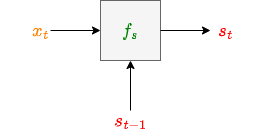
\includegraphics[width=60mm,scale=0.4]{images/rnn_images/transition_diagram.png}
        \end{figure}

        Now, we have two more pieces of our state machine:
        
        \begin{itemize}
            \item \bru{$\mathcal{X}$} is a finite or infinite set of possible \textbf{inputs} \bru{$x$}.
            \item \grn{$f_s$} is the \textbf{transition function}, which moves us from one state to the next, based on the input.
                \begin{equation}
                    \grn{f_s}: \red{\mathcal{S}} \cross \bru{\mathcal{X}} 
                    \rightarrow \red{\mathcal{S}}
                \end{equation}
        \end{itemize}



    \phantom{}

    \subsection{Transition Examples}
        
        Now, we revisit our examples, and consider how they "transition":
        
        \begin{itemize}
            \item The game of chess.
                \begin{itemize}
                    \item The input \bru{$x$} is the \brun{choice} our player makes, \brun{moving one piece} on the chess board according to the \textbf{rules}.
                    
                    \item The transition function \grn{$f_s$} applies this move to our current chess board, and produces a \gren{new chess board}.
                        \begin{itemize}
                            \item If we moved our pawn, the transition function outputs the board \gren{after} that pawn is \gren{moved}.
                        \end{itemize}
                \end{itemize}
                
            \item A ball moving in space, with coordinates.
                \begin{itemize}
                    \item The input \bru{$x$} might represent a \brun{push} changing the ball's velocity.
                    
                    \item The transition function \grn{$f_s$} uses the push to change our \brun{velocity}, and the velocity to change the ball's \brun{position}.
                        \begin{itemize}
                            \item If our ball wasn't moving before, and we \gren{push} it, the new state is \gren{moving} in that direction.
                        \end{itemize}
                \end{itemize}
                
            \item A combination lock with 3 digits.
                \begin{itemize}
                    \item The input \bru{$x$} is you \brun{changing} one of the three digits on the lock: for example, \brun{increasing} the first digit by 3.
                    
                    \item The transition function \grn{$f_s$} applies the \gren{change} you make to the lock.
                        \begin{itemize}
                            \item If the first digit was 2, and you \gren{increase} it by 3, the new first digit is 5.
                        \end{itemize}
                \end{itemize}
        \end{itemize}




    \pagebreak
        
    \subsection{Output}
        
        We now have a system for keeping \textbf{track} of our state, and \textbf{updating} that state: this is a really powerful tool for managing time!
        
        We're still missing something, though: why do we \textbf{care} about our state? Typically, there's some \textbf{result} we actually want from storing our state.
            \note{Just like how in CNNs, convolution wasn't the end goal: it was a transformation to help improve regression/classification.}

        \subsecdiv
        
        Usually, the desired output is more simple than keeping track of everything we want to \textbf{remember}.
            
        \miniex If we're storing a bunch of information about the stock market, and our own money, we might simply return "invest in $X$" or "do not invest in $X$".
        
        The is what we call our \textbf{output}.\\
        
        \begin{definition}
            The \vocab{output} \purp{$y$} represents the \purp{result of our current state}. 
            
            What we use as "output" depends on what we are \gren{trying to predict/compute}.
            
                \begin{itemize}
                    \item Sometimes, the output is the \textbf{only} thing (aside from input) we can \textbf{see}. This happens when the state is \vocab{hidden}!
                \end{itemize}

            \subsecdiv
            
            In other words, while the state \gren{stores} relevant information to keep track of the situation, the \purp{output} is the decision based on this information.
            
            We represent the \textbf{set} of all possible \purp{outputs} as \purp{$\mathcal{Y}$}.
            
            \begin{itemize}
                \item This set can be \textbf{finite} or \textbf{infinite}.
                \item If $y$ is a possible output, we say \purp{$y \in \mathcal{Y}$}.
            \end{itemize}
                
            Our output at time $t$ is \purp{$y_t$}.
        \end{definition}

        Note that we use $y_t$: we don't necessary create a single output at the end of our runtime.
        
        \begin{itemize}
            \item Instead, we continuously create outputs at each timestep.
        \end{itemize}



    \phantom{}

    \subsection{Output Function}
        
        So now, we need to actually \textbf{compute} our output. This will be based on all the data we have \gren{stored} at the time we're asked for an output.

        \begin{itemize}
            \item We don't need to use the input, because the input data is already included in the state.
        \end{itemize}

        We can create an output for each timestep using the \purp{output function}.\\

        \begin{definition}
            The \vocab{output function} \grn{$f_o$} tells us what \purp{output} we get based on our current \redd{state}.
            
            Thus, our \gren{output function} only takes in the \redd{state}. 
            
            \begin{equation*}
                \grn{f_o}(\red{s_t}) = \pur{y_t}
            \end{equation*}
            
            It uses our current information (\redd{state}) to produce a the result we're interested in (\purp{output}).
            
            Using sets, we can write this as:
            
            \begin{equation*}
                \grn{f_o}: \red{\mathcal{S}} \rightarrow \pur{\mathcal{Y}}
            \end{equation*}
        \end{definition}
        
        We visualize this unit as:
        
        \begin{figure}[H]
            \centering
            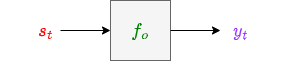
\includegraphics[width=60mm,scale=0.4]{images/rnn_images/output_diagram.png}
        \end{figure}

        This gives us the last two parts of our state machine:
            
        \begin{itemize}
            \item \purp{$\mathcal{Y}$} is a finite or infinite set of possible \textbf{outputs} \purp{$y$}.
            
            \item \grn{$f_o$} is an \textbf{output function}, which gives us our output based on our state.
                \begin{equation}
                    \grn{f_o}: \red{\mathcal{S}} \rightarrow \pur{\mathcal{Y}}
                \end{equation}
        \end{itemize}



    \phantom{}
    
    \subsection{Output Examples}
        
        Again, we go to our examples, and give them outputs, completing our state machines:
        
        \begin{itemize}
            \item The game of chess.
                \begin{itemize}
                    \item The output \purp{$y$} could be many things. But, what do we care about most: \purp{winning}! 
                        \begin{itemize}
                            \item So, \purp{$\mathcal{Y}$} will have four options: "ongoing", "draw", "player 1 win", "player 2 win".
                        \end{itemize}
                        
                    \item The output function \grn{$f_o$} will give us our output. Thus, it represents the \gren{chess rules} for whether there is a winner or a draw.  
                        \begin{itemize}
                            \item So, \grn{$f_o$} looks at a board, and tells us whether someone has won, or there's a draw.
                        \end{itemize}
                \end{itemize}
                
            \item A ball moving in space, with coordinates.
                \begin{itemize}
                    \item We want output \pur{$y$}.
                        \begin{itemize}
                            \item Sometimes, the \purp{output} is the same as the \redd{state}: all we want to know is what's \textbf{happening}!
                            
                            \item In this case, we'll say our \textbf{output is the state}: we return the \purp{position} and \purp{velocity} of the ball.
                                \note{We could have chosen a different output if we had a specific goal in mind!}
                        \end{itemize}
                        
                    \item If our state and output are the same, then the output function \grn{$f_o$} should just \gren{copy} the state it receives!
                        \begin{itemize}
                            \item Our function is the \vocab{identity function}: $\grn{f_o}(\red{s}) = \red{s}$.
                        \end{itemize}
                \end{itemize}
                
            \item A combination lock with 3 digits.
                \begin{itemize}
                    \item We want our output \purp{$y$}. 
                        \begin{itemize}
                            \item Our goal is more clear: we want the combination lock to be \purp{open} or \purp{closed}. So, those are our outputs \purp{$\mathcal{Y}$}.
                        \end{itemize}
                        
                    \item Our function \grn{$f_o$} will tell us the lock is open if the current digits exactly \gren{match the correct sequence}.
                \end{itemize}
        \end{itemize}


    \pagebreak

    \subsection{A Completed State Machine}

        Finally, we can assemble our completed state machine.\\
        
        \begin{definition}
            A \vocab{State Machine} can be formally defined as a collection of several objects 
            
            \begin{equation*}
                (\red{\mathcal{S}}, \bru{\mathcal{X}}, \pur{\mathcal{Y}}, 
                \red{s_0}, \grn{f_s}, \grn{f_o})
            \end{equation*}
            
            We have three sets:
            
            \begin{itemize}
                \item $\red{\mathcal{S}}$ is a finite or infinite \textbf{set} of possible \textbf{states} \red{$s$}.
                
                \item $\bru{\mathcal{X}}$ is a finite or infinite \textbf{set} of possible \textbf{inputs} \bru{$x$}.
                
                \item $\pur{\mathcal{Y}}$ is a finite or infinite \textbf{set} of possible \textbf{outputs} \purp{$y$}.
            \end{itemize}
            
            And components to allow us to transition through time:
            
            \begin{itemize}
                \item $\red{s_0 \in \mathcal{S}}$ is the \textbf{initial state} of the machine. 
                
                \item \grn{$f_s$} is the \textbf{transition function}, which moves us from one state to the next, based on the input.
                    \begin{equation*}
                        \grn{f_s}: \red{\mathcal{S}} \times \bru{\mathcal{X}}
                        \rightarrow \red{\mathcal{S}}
                    \end{equation*}

                \item \grn{$f_o$} is an \textbf{output function}, which gives us our output based on our state.
                    \begin{equation*}
                        \grn{f_o}: \red{\mathcal{S}} \rightarrow \pur{\mathcal{Y}}
                    \end{equation*}
            \end{itemize}
        \end{definition}
        
        We have:
        
        \begin{itemize}
            \item Our \redd{state} to store information,
            \item Our \brun{input} to update information,
            \item Our \purp{output} gives us the result of our information.
        \end{itemize}
        
        And to combine these, we need:
        
        \begin{itemize}
            \item Our \vocab{initial} state,
            \item How to \gren{change} states,
            \item How to \gren{get} an \gren{output}.
        \end{itemize}



    \phantom{}

    \subsection{Using a State Machine}

        How do we work with a state machine? Well, we have all of the tools we need.
        
        We start with out initial state, $\red{s_0}$. For our \textbf{first} timestep, we get a new input: new \textbf{information}. We use this to get a new state.
        
        \begin{equation}
            \red{s_1} = 
            \grn{f_s}(\red{s_0}, \bru{x_1})
        \end{equation}
        
        With this state, we can now get our \textbf{output}.
        
        \begin{equation}
            \pur{y_1} = 
            \grn{f_0}(\red{s_1})
        \end{equation}
        
        We've calculated everything in our \textbf{first} timestep! Now, we can move on to our \textbf{second} timestep, and do the same thing.
        
        In general, we'll repeatedly follow the process:
        
        \begin{equation}
            \red{s_t} = 
            \grn{f_s}(\red{s_{t-1}}, \bru{x_t})
        \end{equation}
        
        \begin{equation}
            \pur{y_t} = 
            \grn{f_o}(\red{s_t})
        \end{equation}
        
        
        \begin{concept}
            To move through time in a state machine, we follow these steps from $t=1$:
            
            \begin{itemize}
                \item Use the \bru{input} and \red{state} to get our \red{new state}.
                    \begin{equation*}
                        \red{s_t} = 
                        \grn{f_s}(\red{s_{t-1}}, \bru{x_t})
                    \end{equation*}
                    
                \item Use the \red{new state} to get our \pur{output}.
                    \begin{equation*}
                        \pur{y_t} = 
                        \grn{f_o}(\red{s_t})
                    \end{equation*}
                    
                \item Increment the time from $t$ to $t+1$.
                
                    \begin{equation*}
                        t_{new} = t_{old} + 1
                    \end{equation*}
                
                \item Repeat.
            \end{itemize}
        \end{concept}



    \phantom{}

    \subsection{Example Run-Through of a State Machine}

        To make this more concrete, we'll build our own simple state machine and run a couple iteration steps.
                
        Suppose you're saving up money to buy something. At each timestep, you gain or lose some money. 
        
        You want to know when you have enough money to buy it. 
            \note{This example is simple enough that you might feel like a state machine is unnecessary. However, this is just for demonstration!}
            
        What are each of the parts of our state machine?
        
        \begin{itemize}
            \item The state $\red{s}$: how much money do we have right now?
            
            \item The input $\bru{x}$: the money we add to our savings.
            
            \item The output $\pur{y}$: we want to know when we have enough money. Maybe our goal is 10 dollars.
            
            \item Initial $\red{s_0}$: we start with 0 dollars.
            
            \item Transition $\grn{f_s}$: we just add the new money to how much we have saved up.
            
                \begin{equation}
                    f_s(\red{s},\bru{x}) = \red{s}+\bru{x}
                \end{equation}
                
            \item Output $\grn{f_o}$: do we have enough money?
            
                \begin{equation}
                    \grn{f_o}(\red{s}) = (\red{s} \geq 10)
                    =
                    \begin{cases}
                        \text{True} & \text{If } s \geq 10 \\
                        \text{False} & \text{Otherwise}
                    \end{cases}
                \end{equation}
        \end{itemize}
        
        We'll run through our state machine for the following input:
        
        \begin{equation}
            \red{X} = [x_1, \; x_2, \; x_3, \; x_4] = [ 4, \; 5, \; 6, \; -7]
        \end{equation}
        
        Let's apply the steps above:
        
        \begin{itemize}
            \item Get new state from (old state, input).
            \item Get output from new state.
            \item Increment time counter.
        \end{itemize}
        
        For our first step, we get:
        
        \begin{equation}
            \begin{matrix}
                \red{s_1} = 4+0 = \red{4} \\
                \\
                \pur{y_1} = ( 4 \geq 10 ) = \text{\pur{False}}
            \end{matrix}
        \end{equation}
        
        For the others, we get:
        
        \begin{equation}
            \begin{matrix}
                \red{s_2} = 9 \\ \pur{y_2} = \text{False}
            \end{matrix}
            \;\; \longrightarrow \;\; 
            \begin{matrix}
                \red{s_3} = 15 \\ \pur{y_3} = \text{True}
            \end{matrix}
            \;\; \longrightarrow \;\; 
            \begin{matrix}
                \red{s_4} = 8 \\ \pur{y_4} = \text{False}
            \end{matrix}
        \end{equation}
        
        Though our transition and output functions might become more complicated, this is the basic idea behind all state machines.




    \phantom{}

    \subsection{State Machine Diagram}
    
        Finally, we'll create a visualization that represents our state diagram.
        
        \subsubsection{Transition Function}
        
            Our \grn{transition function} follows this format:
            
            \begin{equation}
                \red{s_t} = 
                \grn{f_s}(\red{s_{t-1}}, \bru{x_t})
            \end{equation}
            
            We can diagram this component as:
            
            \begin{figure}[H]
                \centering
                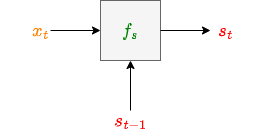
\includegraphics[width=60mm,scale=0.4]{images/rnn_images/transition_diagram.png}
            \end{figure}
            
            Note that the state appears \purp{twice}: once as an input, once as an output.
            
            In the \textit{next} timestep, $s_t$ will be the \textbf{input} to $f_s$, even though it's currently the \textbf{output}.
                \note{If $t=10$, then $s_{10}$ is the output. If $t=11$, then $s_{10}$ is the input!}

            \begin{itemize}
                \item We'll create a way to represent this later.
            \end{itemize}
            
        
        \subsecdiv
        
        \subsubsection{Output Function}
        
            Our \gren{output function} takes in the state we just got from the transition function:
            
            \begin{equation}
                \pur{y_t} = 
                \grn{f_o}(\red{s_t})
            \end{equation}
            
            So, we diagram it accordingly:
            
            \begin{figure}[H]
                \centering
                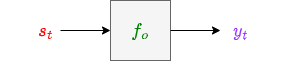
\includegraphics[width=60mm,scale=0.4]{images/rnn_images/output_diagram.png}
            \end{figure}
            
            As we mentioned, the \textbf{output} function takes in the state as its input. 
            
            \begin{itemize}
                \item That means that the \redd{output} of $f_s$, is the \redd{input} of $f_o$.
            \end{itemize}
            
            \begin{figure}[H]
                \centering
                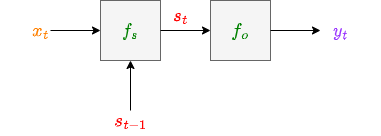
\includegraphics[width=80mm,scale=0.4]{images/rnn_images/state_machine_protodiagram.png}
            \end{figure}
            
        \subsecdiv
        
        \subsubsection{Time Delay}
        
            Only one thing is missing: we know that our current state $\red{s_t}$ needs to be reused \textbf{later}: we'll need it to compute our \textit{new} state $\red{s_{t+1}}$.
            
            We don't want it to \textit{immediately} send the state information back to $f_s$: we only use the function once per timestep. So, we'll \textit{delay} by waiting one time step.
            
            We'll use a little clock symbol to represent this fact.
            
            \begin{figure}[H]
                \centering
                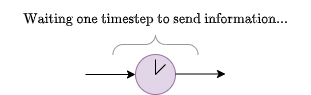
\includegraphics[width=80mm,scale=0.4]{images/rnn_images/clock.png}
            \end{figure}
            
            \begin{notation}
                We can depict a \vocab{state machine} using the following diagram:
                
                \begin{figure}[H]
                    \centering
                    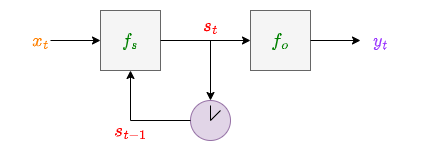
\includegraphics[width=90mm,scale=0.4]{images/rnn_images/state_machine_diagram.png}
                \end{figure}
                
                At every timestep, we use $\bru{x_t}$ and $\red{s_{t-1}}$ to calculate our new state, and our new output.
                
                The circular "clock" element represents our \purp{delay}: $\red{s_t}$ becomes the input to $f_s$ on the \purp{next} timestep.
            \end{notation}




    \pagebreak

    \subsection{Finite State Machines}

        To get used to state machines, we'll start with a simpler, special case, the \textbf{finite state machine}.\\
            
        \begin{definition}
            A \vocab{finite state machine} is a state machine where
            
            \begin{itemize}
                \item The set of states $\red{\mathcal{S}}$
                \item The set of inputs $\bru{\mathcal{X}}$
                \item The set of outputs $\pur{\mathcal{Y}}$
            \end{itemize}
            
            Are all \vocab{finite}. Meaning, the total space of our state machine is \purp{limited}.
            
            Each aspect of our state machine can be put into a finite list of elements: this often makes it easier to \textit{fully} describe our state machine.
        \end{definition}
        
        This seemingly limited tool is more powerful than it seems: \textbf{all computers} can be described as finite state machines!
            \note{Even when a computer seems to be describing "infinite" collections of things, it only has a finite amount of space to represent them.}




    \phantom{}

    \subsection{State Transition Diagrams}

        One nice thing about the simplicity of a finite state machine is that we can represent it \textbf{visually}.
            
        Let's build one up: we'll pick a simple, though not entirely realistic example.
        
        \miniex We have a blanket. It can be in three states: either \blu{wet}, \grn{dry}, or \red{burning}. We can represent each state as a "node".
        
        \begin{figure}[H]
            \centering
            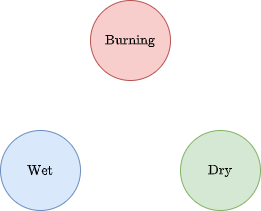
\includegraphics[width=60mm,scale=0.4]{images/rnn_images/std_states.png}
        \end{figure}
        
        \begin{concept}
            In a \vocab{state transition diagram}, states are represented as \purp{nodes}, or points on the graph.
        \end{concept}
        
        We have our states down. The other important thing is our \textbf{transitions}. How do we go between states?
        
        Well, one input could be \textbf{water}: it would stop the blanket from burning. In any case, the blanket will be wet.
        
        \begin{figure}[H]
            \centering
            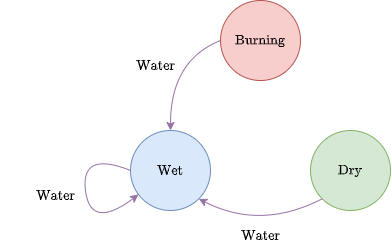
\includegraphics[width=80mm,scale=0.4]{images/rnn_images/std_water.png}
        \end{figure}
        
        Now, we can see: each arrow represents a \textbf{transition} between two states. Each \textbf{input} gets its own transition.\\
        
        \begin{concept}
            In a \vocab{state transition diagram}, transitions are represented as \purp{arrows} between states.
            
            We usually label these with whichever \brun{input} will cause that transition.
        \end{concept}
        
        Also notice that a state can transition to itself: a wet blanket \textbf{stays wet} when you add water.
        
        What if we add \textbf{fire}? That would make a dry blanket \textbf{burn}. But, we could also use it to \textbf{dry off} the wet blanket!
        
        \begin{figure}[H]
            \centering
            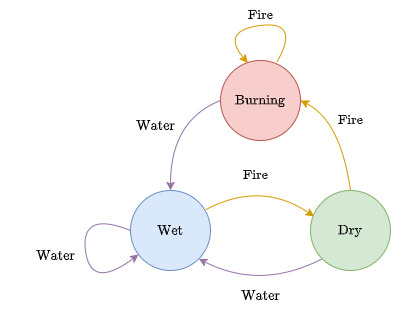
\includegraphics[width=80mm,scale=0.4]{images/rnn_images/std_fire_and_water.png}
        \end{figure}
        
        And now, we have a simple \textbf{state transition diagram}!
            \note{Note that our diagram doesn't show the output. In this case, that's not a problem: the output is the state.}
        
        Each transition, as usual, is based on two things: the \textbf{current} state (where the arrow starts) and the \textbf{input}(which arrow you follow).\\
        
        \begin{definition}
            A \vocab{state transition diagram} is a \purp{graph} of 
            
            \begin{itemize}
                \item Nodes (\red{points}) representing \red{states}
                \item Directed edges (\grn{arrows}) representing \grn{transitions}
            \end{itemize}
            
            Where each input-state pair has one arrow associated with it.
            
            These arrows show one \grn{transition}, with the properties:
            
            \begin{itemize}
                \item The start and end \red{states} represented by the start and the end of the arrow
                \item The \bru{input} that causes this transition is labelled.
            \end{itemize}
            
            This diagram does not have to show the input.
        \end{definition}
        
            \note{If you're not familiar with "nodes" or "edges", don't worry about it! For our purposes, "point" and "arrow" are good enough.}




    \phantom{}

    \subsection{Simplified state transition diagrams: One-input graphs}
        
        One more consideration: the graph above is helpful, but it's a bit \textbf{complicated}. 
        
        In fact, if we added more \textbf{states}, or more \textbf{inputs}, it could get too complicated to read!
        
        Our solution: if a system is too complicated, we create a separate state-transition diagram for \textbf{each input}.
        
        \begin{figure}[H]
            \centering
            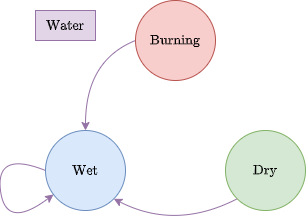
\includegraphics[width=60mm,scale=0.4]{images/rnn_images/std_water_no_label.png}
            \qquad
            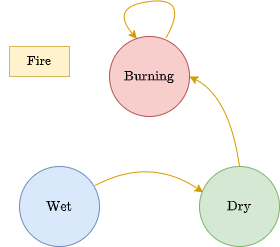
\includegraphics[width=55mm,scale=0.4]{images/rnn_images/std_fire.png}
            
            \caption*{The left diagram only uses \textbf{water} as an input, while the right diagram only uses \textbf{fire} as an input.}
        \end{figure}
        
        Each of our diagrams is much more readable now! Not only do we have less arrows, but we don't have to label each arrow.
        
        As a tradeoff, we have two graphs to keep track of, instead of one. However, this is usually necessary.
            \note{In the next chapter, MDPs, we'll need this!}\\
            
        \begin{concept}
            We can simplify our \vocab{state transition diagrams} by creating a \purp{separate diagram} for each \bru{input}.
            
            This makes it easier to visualize what's going on.
        \end{concept}

    \pagebreak

    \subsection{Linear Time-Invariant Systems (LTI)}

        A wide range of problems can be modelled by a simplified, \gren{linear} version of this system.

        That means we'll work entirely with vectors and matrices: no non-linear functions. 

        \begin{itemize}
            \item Our \redd{states} are all vectors of length $m$.
            \item Our \brun{inputs} are all vectors of length $\ell$.
            \item Our \purp{outputs} are all vectors of length $n$.

            \begin{equation}
                \red{\mathcal{S}} = \RR^m    \qquad\qquad\qquad
                \bru{\mathcal{X}} = \RR^\ell \qquad\qquad\qquad
                \pur{\mathcal{Y}} = \RR^n
            \end{equation}
        \end{itemize}

        To transition between states, we'll \textbf{linearly} combine state $s_{t-1}$, with our input $x_t$: $A$ and $B$ are \gren{matrices}.

        \begin{equation}
            \red{s_{t}} 
            \quad=\quad 
            A\red{s_{t-1}} + B\bru{x_t}
        \end{equation}

        Notice that we \orgg{exclude the offset terms}: this is due to our definition of \textbf{linear}.\\

        \begin{clarification}
            There are two related, but \purp{distinct} definitions for what it means to be \gren{linear}:

            \begin{itemize}
                \item The kind of linear we're more used to: "an equation that draws a line". This is allowed to have an \redd{offset}.

                \begin{equation*}
                    f(x)=W^Tx + W_0
                \end{equation*}

                \item The kind of linearity used in \vocab{linear combinations}, where you're only allowed to \textbf{scale} and \textbf{add} the inputs together: \redd{no offset}.

                \begin{equation*}
                    f(x) = W^Tx
                \end{equation*}
            \end{itemize}

            \subsecdiv

            The latter allows us to use the \gren{linearity} property:

            \begin{equation*}
                f(a+b) = f(a)+f(b) \qquad \qquad f(ca) = cf(a)
            \end{equation*}

            While the former definition, with the offset, does not.
        \end{clarification}

        Our output will simply be a \textbf{linear} scaling of our state: $C$ is a matrix.

        \begin{equation}
            \pur{y_t} 
            \quad=\quad C\red{s_t}
        \end{equation}

        We'll also find a second, interesting property:\\

        \begin{definition}
            \vocab{Time-invariance} is the property of our input having the \gren{same} effect on our system, no matter what \purp{time} we apply it.
        \end{definition}

        Thus, we call this restricted model a \vocab{Linear Time-Invariant System (LTI)}.\\

        \begin{definition}
            A \vocab{Linear Time-Invariant System (LTI)} is a variant of a \purp{state machine}, where

            \begin{itemize}
                \item Our input $x$, state $s$, and output $y$ are all vectors

                \begin{equation*}
                    \red{\mathcal{S}} = \RR^m    \qquad\qquad\qquad
                    \bru{\mathcal{X}} = \RR^\ell \qquad\qquad\qquad
                    \pur{\mathcal{Y}} = \RR^n
                \end{equation*} 
                
                \item Our transition and output functions are linear (with $A$, $B$, and $C$ being matrices)
                    \begin{equation*}
                        \red{s_t} 
                        \quad=\quad 
                        \grn{f_s}\Big(\red{s_{t-1}},\bru{x_t}\Big) 
                        \quad=\quad 
                        A\red{s_{t-1}} + B\bru{x_t}
                    \end{equation*}

                    \begin{equation*}
                        \pur{y_t} 
                        \quad=\quad \grn{f_o}\Big(\red{s_t}\Big) 
                        \quad=\quad C\red{s_t}
                    \end{equation*}
            \end{itemize}
        \end{definition}

        We can depict this with a modified version of our state machine diagram from above:

        \begin{figure}[H]
            \centering
            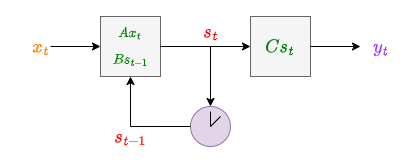
\includegraphics[width=100mm,scale=0.4]{images/rnn_images/lti_diagram.png}
        \end{figure}

        

        This kind of model is often an excellent approximation of simple systems in physics, signals, and other sciences.
